\chapter{Introduction}

\section{Immunoglobulin recombination}

% TODO: source these figures
\begin{figure}
  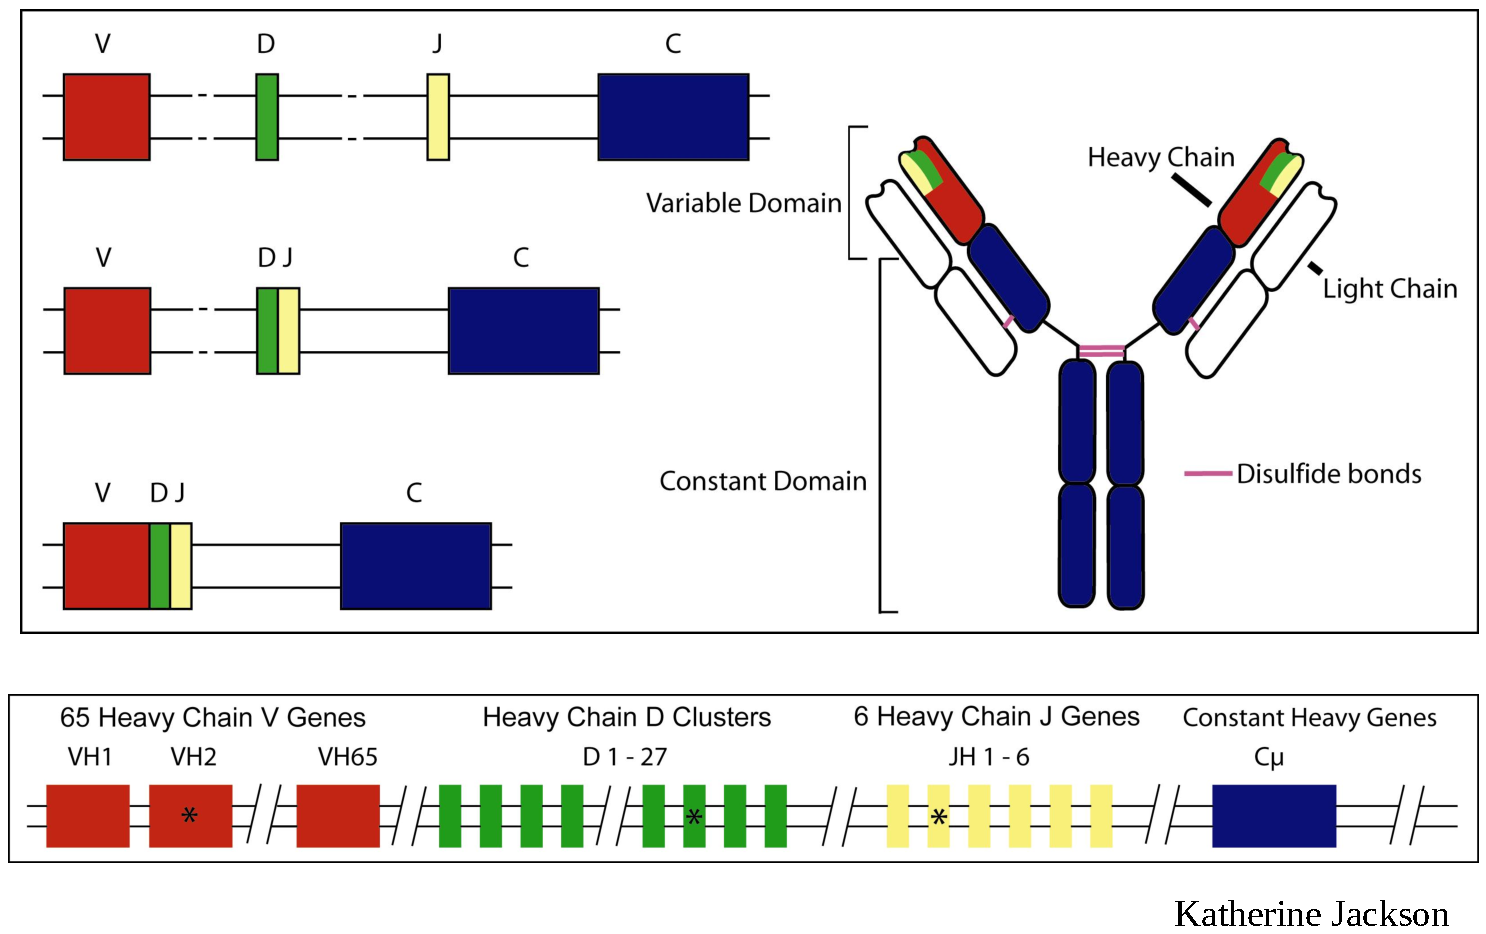
\includegraphics[width=\textwidth]{rearrangement.pdf}
  \caption{The IGHV, IGHD and IGHJ gene recombination process}
  \label{fig:combination}
\end{figure}
\begin{figure}
  \centering
  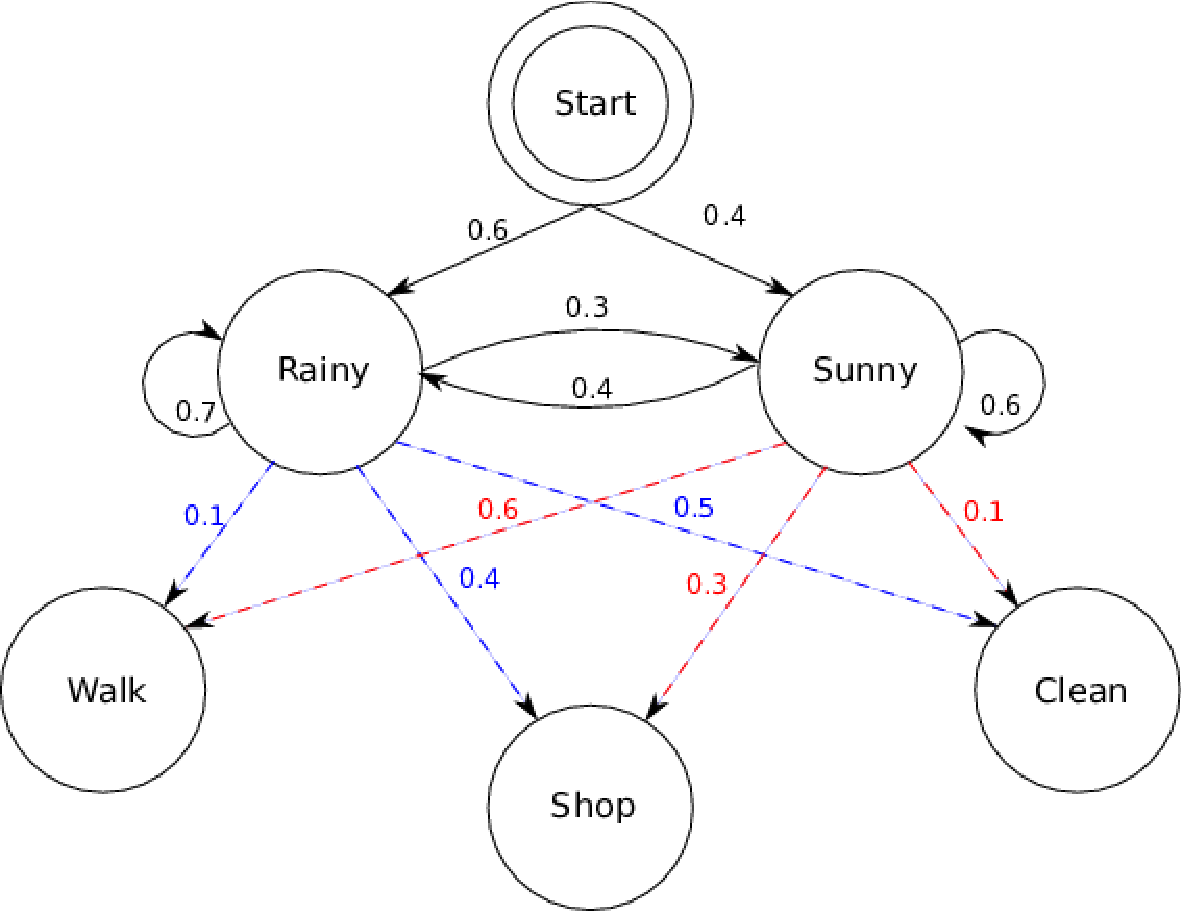
\includegraphics[width=12cm]{hmm-graph.pdf}
  \caption{An example Hidden Markov Model \autocite{wiki-hmm}}
  \label{fig:hmm}
\end{figure}

The human immune system faces many challenges when dealing with foreign pathogens invading the body. One of them is identifying and classifying antigens that are not only vastly diverse, but also constantly mutating and evolving.

It does so by creating immunoglobulins (also called antibodies) whose job is to identify and bind to certain antigens, effectively marking them for destruction by the rest of the immune system. The process, by necessity is highly selective - a given antibody will only bind to a very specific antigen.

However, to deal with the highly diverse and evolving nature of foreign antigens, antibodies must mutate very rapidly. This allows them to be as diverse as the antigens they face, and adapt to bind to newly encountered pathogens.

The process (essentially randomly) selects 3 germline genes from a repertoire in the person's DNA  potentially consisting of between 38 and 45 IGHV genes \autocite{lefranc05, li02}, 23 IGHD genes \autocite{lee06} and 6 IGHJ \autocite{ravetch81} genes. These selected genes are then mutated (adding, removing or changing nucleotides) to generate further diversity. The antibodies that successfully bind to the antigen emit a chemical signal, which then encourages the production of similar antibodies. This entire process is illustrated in \autoref{fig:combination} and explained in more detail by Ga\"{e}ta \textit{et al.}\autocite{iHMMuneAlign}.

\section{iHMMuneAlign}

As a result of this gene recombination and mutation process, the germline genes often don't provide much information on rearranged genes found in the B-Cells that create the antibodies themselves.

Developed in 2007 by a team of researchers at UNSW, iHMMuneAlign attempts to simulate the process of immunoglobulin gene rearrangement.\autocite{iHMMuneAlign}.It represents the recombination process of immunoglobulin heavy chain genes as a hidden Markov model, and then uses it to find the most probable set of germline genes that created the rearranged gene.

First, it selects the most likely IGHV germline gene from its repertoire of possible V genes, using the NCBI's Basic Local Alignment Search Tool (BLAST) \autocite{blast}. It then constructs a Hidden Markov Model with that IGHV gene, and all the possible IGHD and IGHJ genes, together with other states representing the somatic mutation.

It then uses the Viterbi algorithm to determine the most likely sequence of states (genes and their mutations) that caused the observed emissions (the rearranged sequence given as input).

\section{Hidden Markov Models}

A Hidden Markov Model is effectively a Markov Chain, where the states cannot be observed directly. They are used in a wide variety of machine learning applications, including speech recognition \autocite{hmm}.

An example of a HMM is shown in \autoref{fig:hmm}. In this example, if the sequence of emissions \texttt{Walk} was observed, the probability of it being \texttt{Sunny} is
$$I\left(\textnormal{Sunny}\right) \times E(\textnormal{Sunny},\textnormal{Walk}) = 0.4 \times 0.6 = 0.24$$
and the probability of it being Rainy is
$$I(\textnormal{Rainy}) \times E(\textnormal{Rainy,Walk}) =
0.6 \times 0.1 = 0.06$$
where $I(X)$ is the initial probability of $X$ and $E(X,Y)$ is the emission probability of state $Y$ in state $X$.

If \texttt{Walk, Clean} were observed. The probability of it having been Rainy then Sunny is
$$
  I(\textnormal{Rainy})
  \times
  E(\textnormal{Rainy,Walk})
  \times
  T(\textnormal{Rainy, Sunny})
  \times
  E(\textnormal{Sunny, Clean})
  =
  0.6 \times 0.1 \times 0.3 \times 0.1
  = 0.0018
$$
where $T(X, Y)$ is the probability of transitioning from state $X$ to state $Y$.

The Viterbi algorithm uses dynamic programming to recursively explore these probabilities, and selects the sequence of states with the highest probability at the end.

\chapter{Analysis}
Since the high level aim of this project is to improve the performance of iHMMuneAlign, it was necessary to analyse the existing implementation in order to gain insight into its structure, as well as to create realistic aims.

\section{Run Time}
\begin{figure}
  \centering
  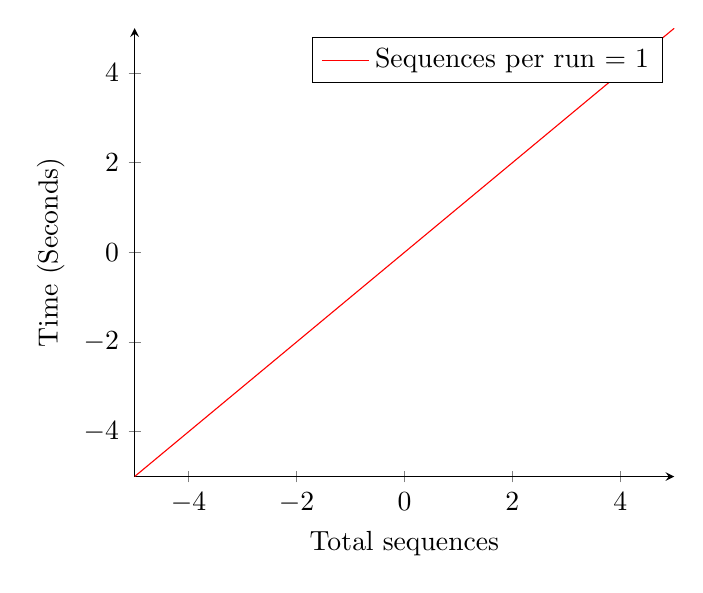
\begin{tikzpicture}
    \begin{axis}[
      axis lines = left,
      xlabel = Total sequences,
      ylabel = Time (Seconds),
      cycle list name=color list
    ]

      \addplot [
    color = red
  ]{x};
  \addlegendentry{Sequences per run = 1}

    \end{axis}
  \end{tikzpicture}
  \caption{Total time taken (in seconds) to process the number of sequences (Wall-clock time). $n$ is the number of sequences per invocation of the program}
  \label{fig:runtime}
\end{figure}
\begin{figure}
  \centering
  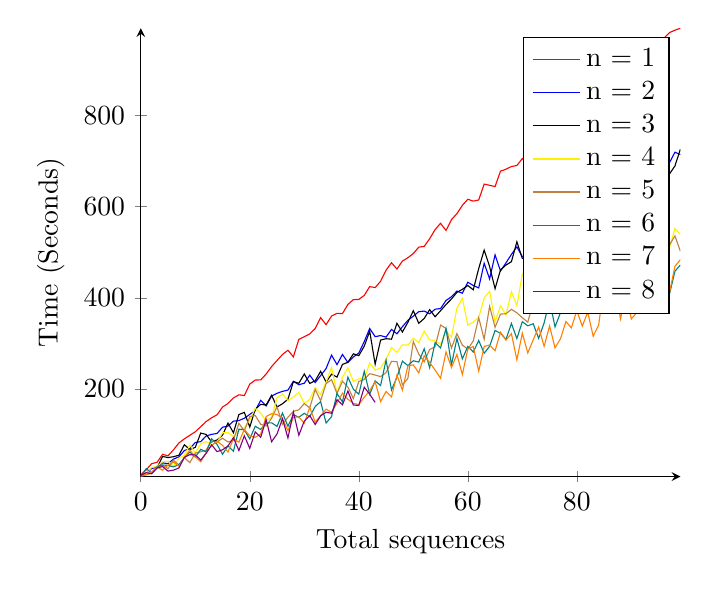
\begin{tikzpicture}
    \begin{axis}[
      axis lines = left,
      xlabel = Total sequences,
      ylabel = Time (Seconds),
      cycle list name=color list
    ]

      \addplot coordinates {(0, 12.217) (1, 22.953) (2, 36.363) (3, 39.593) (4, 56.95) (5, 53.69) (6, 66.68299999999999) (7, 81.873) (8, 90.867) (9, 98.613) (10, 106.4) (11, 117.517) (12, 128.83) (13, 137.047) (14, 143.703) (15, 160.553) (16, 168.377) (17, 180.477) (18, 187.363) (19, 185.833) (20, 210.883) (21, 219.71699999999998) (22, 220.13) (23, 232.94) (24, 249.157) (25, 262.58) (26, 275.7) (27, 285.027) (28, 270.68) (29, 308.963) (30, 314.687) (31, 320.873) (32, 332.613) (33, 356.477) (34, 341.09000000000003) (35, 360.003) (36, 365.943) (37, 365.387) (38, 385.39300000000003) (39, 395.933) (40, 396.477) (41, 405.25) (42, 424.597) (43, 422.443) (44, 436.16700000000003) (45, 460.503) (46, 476.877) (47, 463.137) (48, 480.507) (49, 487.743) (50, 497.067) (51, 511.003) (52, 512.73) (53, 529.41) (54, 549.517) (55, 563.347) (56, 547.543) (57, 571.413) (58, 584.523) (59, 602.627) (60, 616.06) (61, 611.88) (62, 614.48) (63, 649.237) (64, 646.577) (65, 643.893) (66, 677.667) (67, 681.787) (68, 687.717) (69, 689.95) (70, 705.2) (71, 693.857) (72, 715.217) (73, 730.85) (74, 745.593) (75, 762.927) (76, 794.46) (77, 780.163) (78, 791.54) (79, 780.433) (80, 819.9) (81, 819.49) (82, 813.703) (83, 823.697) (84, 866.76) (85, 856.563) (86, 845.58) (87, 879.407) (88, 909.97) (89, 925.833) (90, 921.067) (91, 912.287) (92, 918.253) (93, 962.357) (94, 948.447) (95, 953.217) (96, 969.237) (97, 981.413) (98, 986.54) (99, 990.897)};
\addlegendentry{n = 1}
\addplot coordinates {(0, 8.7) (1, 14.503) (2, 25.713) (3, 28.793) (4, 38.187) (5, 36.447) (6, 46.453) (7, 51.43) (8, 65.233) (9, 69.39) (10, 82.887) (11, 84.777) (12, 97.303) (13, 100.703) (14, 102.743) (15, 116.34) (16, 118.917) (17, 129.63) (18, 130.887) (19, 135.963) (20, 144.46) (21, 152.637) (22, 175.25) (23, 163.117) (24, 184.617) (25, 190.71) (26, 194.923) (27, 197.757) (28, 216.973) (29, 209.463) (30, 212.79) (31, 230.393) (32, 214.26) (33, 229.447) (34, 244.95) (35, 274.413) (36, 253.57) (37, 275.78) (38, 258.31) (39, 270.367) (40, 278.867) (41, 304.047) (42, 332.837) (43, 314.85699999999997) (44, 317.183) (45, 313.83) (46, 330.71) (47, 321.123) (48, 336.677) (49, 350.563) (50, 359.64300000000003) (51, 369.623) (52, 370.87) (53, 365.053) (54, 374.947) (55, 376.5) (56, 394.133) (57, 402.317) (58, 414.763) (59, 409.937) (60, 434.087) (61, 427.023) (62, 421.61) (63, 475.747) (64, 441.47) (65, 494.077) (66, 458.76) (67, 476.6) (68, 495.01) (69, 511.91) (70, 490.02) (71, 487.42) (72, 508.64) (73, 510.377) (74, 535.23) (75, 549.197) (76, 533.417) (77, 531.57) (78, 578.523) (79, 545.643) (80, 555.7) (81, 567.35) (82, 598.037) (83, 603.117) (84, 641.99) (85, 609.673) (86, 610.703) (87, 613.213) (88, 601.08) (89, 622.013) (90, 622.207) (91, 679.66) (92, 675.133) (93, 660.263) (94, 648.577) (95, 704.793) (96, 675.113) (97, 696.167) (98, 719.123) (99, 713.793)};
\addlegendentry{n = 2}
\addplot coordinates {(0, 11.25) (1, 13.16) (2, 15.987) (3, 27.597) (4, 52.22) (5, 49.83) (6, 51.69) (7, 54.993) (8, 77.893) (9, 67.533) (10, 72.12) (11, 103.547) (12, 100.453) (13, 83.99) (14, 88.467) (15, 98.89) (16, 125.493) (17, 104.243) (18, 144.127) (19, 148.833) (20, 116.74000000000001) (21, 155.673) (22, 166.48) (23, 165.077) (24, 186.327) (25, 160.703) (26, 167.767) (27, 177.7) (28, 216.313) (29, 212.76) (30, 232.963) (31, 212.403) (32, 218.1) (33, 238.793) (34, 215.25) (35, 232.567) (36, 226.297) (37, 253.95) (38, 258.67) (39, 277.15) (40, 273.217) (41, 293.98) (42, 326.903) (43, 254.443) (44, 307.37) (45, 310.337) (46, 309.273) (47, 343.983) (48, 325.03) (49, 346.10699999999997) (50, 371.667) (51, 344.18) (52, 354.68) (53, 374.087) (54, 358.47) (55, 371.683) (56, 385.22) (57, 397.413) (58, 411.8) (59, 418.567) (60, 427.013) (61, 417.557) (62, 464.213) (63, 504.637) (64, 468.403) (65, 419.983) (66, 461.203) (67, 471.82) (68, 479.1) (69, 522.757) (70, 486.383) (71, 486.383) (72, 490.717) (73, 461.02) (74, 494.377) (75, 524.643) (76, 483.14) (77, 544.813) (78, 524.543) (79, 514.187) (80, 553.7) (81, 596.79) (82, 546.727) (83, 637.483) (84, 558.65) (85, 557.59) (86, 577.55) (87, 610.47) (88, 630.747) (89, 593.66) (90, 570.61) (91, 623.413) (92, 603.357) (93, 645.063) (94, 637.43) (95, 701.787) (96, 601.47) (97, 671.563) (98, 688.957) (99, 725.823)};
\addlegendentry{n = 3}
\addplot coordinates {(0, 10.597) (1, 13.827) (2, 28.25) (3, 30.2) (4, 40.583) (5, 41.867) (6, 30.507) (7, 48.593) (8, 54.55) (9, 77.373) (10, 59.687) (11, 79.98) (12, 84.907) (13, 78.31700000000001) (14, 83.543) (15, 104.13300000000001) (16, 104.9) (17, 95.61699999999999) (18, 109.36699999999999) (19, 115.087) (20, 132.377) (21, 157.863) (22, 147.1) (23, 130.523) (24, 138.22) (25, 180.91) (26, 189.14) (27, 174.16) (28, 182.45) (29, 193.127) (30, 168.46699999999998) (31, 177.243) (32, 203.313) (33, 188.22) (34, 215.167) (35, 247.55) (36, 191.543) (37, 225.743) (38, 246.643) (39, 216.727) (40, 222.393) (41, 223.003) (42, 257.233) (43, 241.39) (44, 246.227) (45, 264.927) (46, 290.84000000000003) (47, 280.46) (48, 296.653) (49, 296.55) (50, 311.333) (51, 301.93) (52, 326.783) (53, 307.8) (54, 305.523) (55, 298.08299999999997) (56, 327.467) (57, 314.06) (58, 377.163) (59, 398.81) (60, 340.13) (61, 346.637) (62, 357.31) (63, 399.823) (64, 414.277) (65, 347.023) (66, 382.523) (67, 362.13) (68, 413.387) (69, 382.713) (70, 452.193) (71, 428.817) (72, 424.397) (73, 400.49) (74, 391.97) (75, 453.883) (76, 463.733) (77, 426.153) (78, 470.477) (79, 473.077) (80, 467.94) (81, 483.87) (82, 480.22) (83, 505.577) (84, 495.697) (85, 533.027) (86, 522.72) (87, 541.047) (88, 503.373) (89, 548.897) (90, 569.56) (91, 504.91700000000003) (92, 534.5) (93, 587.93) (94, 517.203) (95, 548.0) (96, 561.523) (97, 509.113) (98, 552.057) (99, 539.197)};
\addlegendentry{n = 4}
\addplot coordinates {(0, 8.307) (1, 12.41) (2, 15.677) (3, 27.307) (4, 32.903) (5, 25.57) (6, 43.853) (7, 33.84) (8, 49.69) (9, 38.63) (10, 59.633) (11, 62.503) (12, 66.237) (13, 85.987) (14, 83.803) (15, 92.28) (16, 84.0) (17, 87.643) (18, 124.857) (19, 108.41) (20, 139.553) (21, 142.163) (22, 122.79) (23, 118.913) (24, 135.867) (25, 161.367) (26, 122.527) (27, 138.15) (28, 151.06) (29, 154.47) (30, 168.22) (31, 158.417) (32, 199.273) (33, 174.46) (34, 211.9) (35, 220.637) (36, 190.42) (37, 217.15699999999998) (38, 204.337) (39, 179.153) (40, 216.697) (41, 220.773) (42, 233.787) (43, 230.713) (44, 227.24) (45, 236.027) (46, 260.817) (47, 259.9) (48, 209.213) (49, 223.03300000000002) (50, 304.067) (51, 276.697) (52, 259.687) (53, 286.78) (54, 292.677) (55, 340.25) (56, 332.93) (57, 289.9) (58, 321.513) (59, 296.15999999999997) (60, 287.69) (61, 305.547) (62, 356.42) (63, 309.373) (64, 381.467) (65, 335.383) (66, 364.3) (67, 365.1) (68, 374.77) (69, 367.087) (70, 356.457) (71, 346.527) (72, 389.673) (73, 424.407) (74, 387.483) (75, 451.77) (76, 392.367) (77, 376.103) (78, 414.447) (79, 431.453) (80, 414.747) (81, 423.89) (82, 409.35) (83, 471.757) (84, 431.487) (85, 471.063) (86, 462.96) (87, 475.05) (88, 477.64) (89, 486.307) (90, 493.873) (91, 462.43) (92, 458.7) (93, 516.497) (94, 467.827) (95, 503.057) (96, 525.62) (97, 515.957) (98, 535.747) (99, 501.85)};
\addlegendentry{n = 5}
\addplot coordinates {(0, 8.19) (1, 25.637) (2, 15.877) (3, 30.51) (4, 33.557) (5, 32.67) (6, 29.333) (7, 34.203) (8, 49.313) (9, 61.893) (10, 50.667) (11, 67.813) (12, 62.023) (13, 91.09) (14, 78.4) (15, 56.99) (16, 75.577) (17, 63.5) (18, 112.137) (19, 110.53999999999999) (20, 90.857) (21, 118.5) (22, 111.45) (23, 125.397) (24, 126.007) (25, 118.18299999999999) (26, 147.32999999999998) (27, 118.61699999999999) (28, 143.63) (29, 138.317) (30, 146.707) (31, 139.35) (32, 161.86) (33, 172.45) (34, 125.447) (35, 139.53300000000002) (36, 190.273) (37, 171.93) (38, 225.96699999999998) (39, 199.66) (40, 188.72) (41, 238.933) (42, 188.68) (43, 217.96) (44, 207.65) (45, 263.64) (46, 198.067) (47, 225.737) (48, 261.23) (49, 251.403) (50, 261.983) (51, 259.16) (52, 288.283) (53, 246.79) (54, 301.787) (55, 290.343) (56, 332.503) (57, 252.737) (58, 310.953) (59, 266.027) (60, 293.35) (61, 281.227) (62, 306.347) (63, 278.45) (64, 293.61) (65, 328.303) (66, 322.267) (67, 308.807) (68, 343.847) (69, 310.64300000000003) (70, 347.693) (71, 338.613) (72, 343.157) (73, 311.09) (74, 344.957) (75, 394.10699999999997) (76, 336.337) (77, 367.203) (78, 382.54) (79, 393.617) (80, 425.35) (81, 402.947) (82, 409.12) (83, 385.4) (84, 452.063) (85, 458.657) (86, 429.84) (87, 459.82) (88, 422.84) (89, 419.923) (90, 399.52) (91, 425.613) (92, 504.123) (93, 440.5) (94, 461.067) (95, 465.8) (96, 420.5) (97, 408.123) (98, 458.203) (99, 471.85699999999997)};
\addlegendentry{n = 6}
\addplot coordinates {(0, 11.047) (1, 11.983) (2, 18.177) (3, 29.047) (4, 22.05) (5, 33.35) (6, 39.897) (7, 30.757) (8, 49.37) (9, 66.267) (10, 51.41) (11, 40.68) (12, 60.427) (13, 76.23) (14, 85.517) (15, 76.627) (16, 61.917) (17, 91.273) (18, 83.64) (19, 111.43) (20, 97.483) (21, 94.31) (22, 100.997) (23, 139.763) (24, 145.85) (25, 144.437) (26, 135.087) (27, 108.917) (28, 138.043) (29, 138.817) (30, 124.883) (31, 159.97) (32, 127.637) (33, 141.62) (34, 155.93) (35, 148.983) (36, 169.27) (37, 191.02) (38, 177.773) (39, 168.633) (40, 166.013) (41, 181.91) (42, 196.45) (43, 216.1) (44, 172.527) (45, 194.727) (46, 182.77) (47, 230.63) (48, 197.703) (49, 250.547) (50, 253.05) (51, 235.35) (52, 273.227) (53, 258.123) (54, 241.617) (55, 223.7) (56, 281.283) (57, 247.31) (58, 275.93) (59, 231.757) (60, 287.69) (61, 293.247) (62, 239.287) (63, 293.317) (64, 296.63) (65, 284.03) (66, 324.62) (67, 307.113) (68, 321.413) (69, 264.093) (70, 322.493) (71, 279.183) (72, 307.893) (73, 336.013) (74, 293.513) (75, 338.467) (76, 290.253) (77, 310.173) (78, 348.0) (79, 334.22) (80, 371.99) (81, 337.903) (82, 368.623) (83, 315.927) (84, 339.957) (85, 427.467) (86, 430.837) (87, 435.117) (88, 353.653) (89, 405.65999999999997) (90, 353.757) (91, 367.7) (92, 406.92) (93, 426.853) (94, 426.393) (95, 473.207) (96, 434.437) (97, 411.87) (98, 469.08) (99, 483.7)};
\addlegendentry{n = 7}
\addplot coordinates {(0, 10.617) (1, 16.88) (2, 14.27) (3, 27.283) (4, 30.047) (5, 20.167) (6, 22.257) (7, 26.98) (8, 50.56) (9, 56.123) (10, 55.72) (11, 44.34) (12, 59.19) (13, 77.807) (14, 62.833) (15, 66.803) (16, 75.14) (17, 93.4) (18, 65.13) (19, 97.493) (20, 69.907) (21, 106.06) (22, 94.15299999999999) (23, 133.02) (24, 84.503) (25, 101.66) (26, 135.047) (27, 92.777) (28, 149.66) (29, 98.7) (30, 129.977) (31, 141.927) (32, 122.25) (33, 141.237) (34, 149.207) (35, 146.877) (36, 176.71) (37, 165.37) (38, 195.557) (39, 165.07) (40, 164.027) (41, 204.01) (42, 188.747) (43, 170.777)};
\addlegendentry{n = 8}

    \end{axis}
  \end{tikzpicture}
  \caption{Total time spent doing work by each CPU on behalf of the process during execution (CPU Time). $n$ is the number of sequences per invocation of the program}
  \label{fig:usertime}
\end{figure}

One of the primary attributes of performance, is run time. We begin by measuring the run time of the existing implementation and -more importantly- how it grows with workload.

The current implementation consists of a Java executable and a shell script, to allow running in batches. The Java executable (which does the actual processing) takes a range of input from the script and attempts to process that many in parallel. It then invokes Java program after breaking up the entire range into batches of a given size.

Since we are interested in the rate the total runtime changes with workload as well with increasing parallelism, both were measured. It was run with a total workload ranging from 1 sequences to 100 sequences, with batch size ranging from 1 to 8. The results are shown in \autoref{fig:runtime}.

Note that this was performed on a machine with an AMD Phenom II 1090T (6-core) processor, 8GB of RAM and a solid state hard drive.

%TODO: add reference about schedulers
\subsection{Interpretation of Results}
\label{sec:threadbench}
With a batch size of 1, the expected linear increase was present. However, increasing the batch size shows a more sporadic decrease in runtime. There could be a number of causes for this, including the threads being assigned different CPUs by the scheduler on some runs but not others, increasing cache misses. Nonetheless, it wasn't investigated further, due to time constraints, and the fact that we didn't need such high accuracy for this test. However, there is an overall decrease in total execution time, as the batch size increases.

This suggests that the existing implementation is concurrent, and will utilize all the available processing power on the CPU. However, that should have diminishing returns once the amount of threads exceeds the total number of CPU cores on the machine, which is not the case here - execution time continues to decrease at roughly the same pace as $n$ increases.

Looking at the total CPU time spent on the process, rather than total execution time provided a theory (which was later confirmed in Section \ref{sec:threadprof}, on page \pageref{sec:threadprof}) to explain this behaviour.
For each invocation of the Java program, there is a significant amount of overhead. For example, the Java Virtual Machine (JVM) needs to be initialized, it needs to load the program, analyse and perform any JIT compilation (Just-in-Time compilation, to improve execution time \autocite{jit}). The program also needs to read in the repertoire data files for each gene and process them. On top of all that, any data that are being cached by the operating system on behalf of the program will be invalidated. Since this only needs to be done once per batch, as the batch sizes increases (and the number of batches decrease), this overhead also decreases.

This is clearly apparent in \autoref{fig:usertime}, which shows that the total work done by the program to process all the sequences is reduced significantly as the $n$ increases.

Comparing the total executable time (wall clock time) and the total CPU time of each run shows, that there was roughly double the CPU time as execution time. This indicates that the program has 2 threads of execution, but that it doesn't increase threads with workload.


\section{Profiling}
\begin{figure}[p]
  \centering
  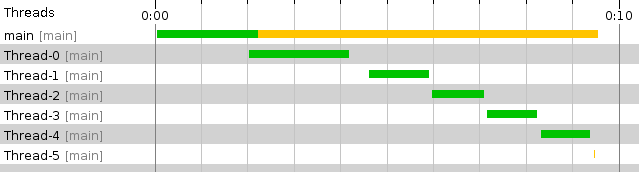
\includegraphics[width=\textwidth]{threads-graph.png}
  \caption{Time spent by each thread;
  running (\protect
\includegraphics{jprofiler_images/ff00c400_bff000000.png}) and
  waiting (\protect
\includegraphics{jprofiler_images/ffffc400_bff000000.png})}
  \label{fig:threadgraph}
\end{figure}
\begin{figure}[p]
  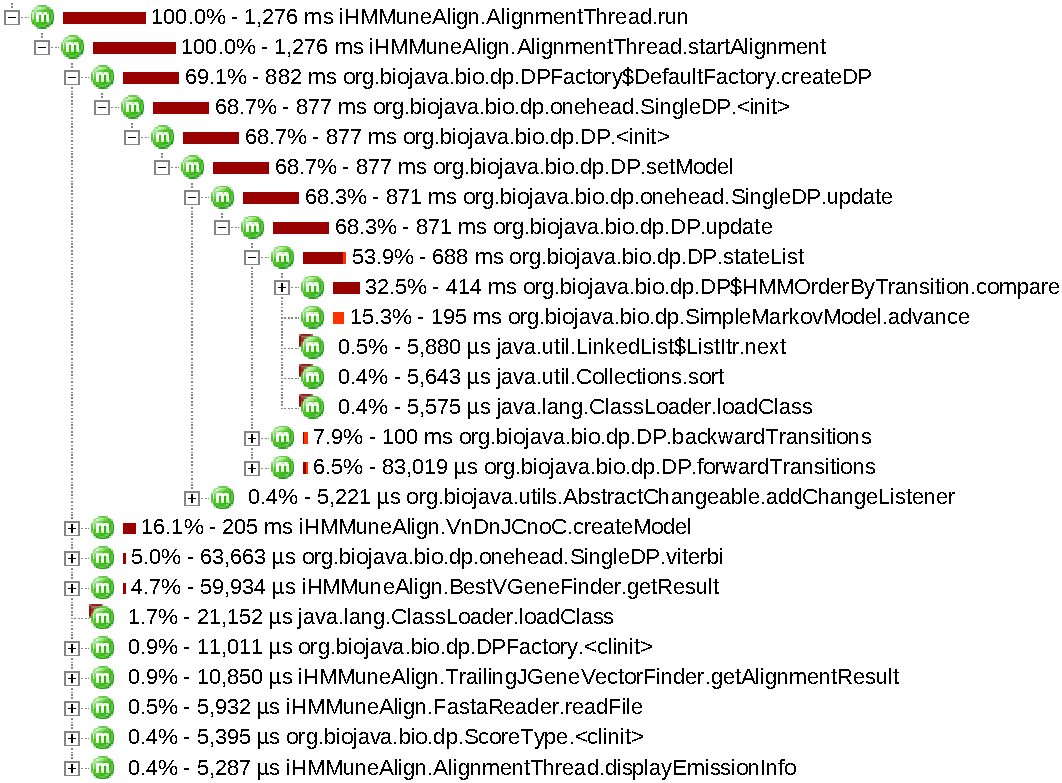
\includegraphics[width=\textwidth]{call-tree.pdf}
 \caption{The call graph generated by jProfiler, for a single run of iHMMuneAlign}
 \label{fig:callgraph}
\end{figure}
In order to determine the most appropriate approaches for improving performance and overcoming the limitations of the original implementation, further analysis is required. Specifically, we are interested in which parts of the program consume the most CPU time and memory, as well as how they increase with the workload.

The method for collecting this data is called profiling. Since the original implementation of iHMMuneAlign was written in Java, we can use various interfaces in the Java Virtual Machine (JVM) to gather this data. The JVM has an interface called Java Native Interface (JNI)\autocite{jni}, that allows external programs and native libraries (usually written in C/C++) to interact with Java objects. Alongside that, from Java version 1.5 onwards, the JVM also provides another interface, called Java Virtual Machine Tool Interface (JVMTI), which allows external tools to be notified as certain events (such as object allocation, method call) occur during execution.

In \autoref{fig:callgraph}, the data for a run of iHMMuneAlign with 6 sequences, instrumented by jProfiler \autocite{jprofiler} (a profiler implemented with the above method) is shown.

\subsection{CPU Call Graph}
\label{sec:cpuprof}
Figure \autoref{fig:callgraph} shows the time, and the percentage of total execution time spent in each method invocation of a single execution of iHMMuneAlign.

It begins with the equivalent of the \texttt{main()} function for a thread using Java's built in threading library - \texttt{Thread.run()}, which in turn calls \texttt{startAlignment()}. However, it becomes immediately apparent that the majority of execution time from there is spent in the BioJava library.

68\% of total execution time is spent constructing a \texttt{org.biojava.bio.dp.SingleDP} object, which will allow various algorithms (including Viterbi) to be performed. It takes a \texttt{org.biojava.bio.dp.MarkovModel} object, which represents the Markov Model, and converts it to its own internal format. This conversion involves sorting all the states, which is what 53.9\% of the whole program's execution time is spent on.

For our purposes, this conversion is unnecessary, as we can generate the states ourselves, and can easily do so in the order necessary to run Viterbi on them. The actual call to the \texttt{DP.viterbi()} method, which actually runs the Viterbi algorithm to determine the most likely sequence of states, takes only 5.0\% of the total execution time.

\subsection{Threads}
\label{sec:threadprof}
An important aspect of the existing implementation is its threading model - i.e. how it distributes the workload between multiple threads of execution (which can then run on multiple CPUs or CPU cores). Since we already determined in Section \ref{sec:threadbench} that it does indeed use multiple threads, we need to look more closely at exactly how it does so.

For this, we have our profiler record events in the \texttt{java.util.concurrent} package, which include thread creation, destruction and blocking (waiting for another thread to complete). The results of this, shown in \autoref{fig:threadgraph} confirm our earlier hypothesis. The program has two threads active most of the time; one processing the gene, and one (main thread) waiting for it to complete, before starting the next one.

The fact that they use a threading library indicates that the original authors intended to make iHMMuneAlign a concurrent program, processing multiple gene sequences in parallel. While their architecture would have been less performance efficient than using a thread pool (as they have to pay the cost of thread creation and destruction for each sequence), it would still have caused a notable improvement if they allowed the threads to execute in parallel.

Nonetheless, the fact that the main thread doesn't create each thread until its predecessor terminates indicates said efforts of parallelism were abandoned. It is widely regarded in industry that concurrent programming is rather difficult and the original authors most likely deemed completing the project was more prudent than making it concurrent.

No further investigation was done to determine what would need to be done in order to make the current implementation concurrent, as it will most likely be rewritten for this project.

\chapter{Proposed Solution}

\section{Re-implementing From Scratch}

Based on the above analysis, it is clear that the original codebase has many pitfalls, and limitations that make it difficult to proceed further.

\subsection{Code Maintainability}
Most of the logic for processing a gene sequence is contained in the \begin{center}
  \texttt{AlignmentThread.startAlignment()}
\end{center}
method, which over 2000 lines long. The project doesn't use any revision control systems, and the fact it is littered with commented out code most likely indicates that it didn't do so at any point in the past either.

There are no unit tests that cover most of the program logic, and it would be difficult to write any, since the logic hasn't been split up. This makes it rather difficult to make changes, without introducing any new subtle bugs, or undesired behaviour.

The original authors are no longer available to provide assistance for understanding their codebase, and the style guide they followed (or lack thereof) makes it difficult to read and follow.

It is understandable that the original authors did not prioritize long term code maintainability, as they could have been rushed for time, or they may have deemed it unlikely their could would be used and maintained 7 years later.

\subsection{Concurrency / Thread Safety}

Concurrency must be considered from the very early design decisions onwards, for a program to be efficient and parallel. The fact the original authors abandoned their efforts for parallelism indicates that there may have been concurrency bugs, like race conditions \autocite{raceconditions} that are very difficult to trace.

Access to shared data must be carefully controlled, and synchronized to avoid data corruption (and race conditions). The potentially high overhead of synchronization should lead to program structure designs where shared data between threads is minimal. In addition, the thread safety of any libraries used must be carefully considered - if a class is not thread safe, it shouldn't be shared  between threads; and if a class is not re-entrant, there shouldn't even be separate instances in different threads.

\subsection{Libraries and Language}
Some of the libraries that the original authors used have since been deprecated. The specific libraries are mentioned in more detail below. Considering that some libraries account for most of the performance inefficiencies of the program (as shown in Section \ref{sec:cpuprof}), they will certainly need to be replaced. Since the libraries' APIs heavily influenced the structure of the code, replacing them while maintaining the existing code structure will be a difficult task.

There is also the language itself to consider: Java programs tend to be 2-3 times slower than their equivalent C++ counterparts, and even more so in CPU bound tasks like this \autocite{qtvjava}. Reimplementing from scratch will allow us to do so in a different language. C++ is a good candidate - it is quite popular for constructing large scale, high performance applications \autocite{cpp}; it contains high concepts from high level languages, while still allowing for low level optimizations, including memory management.

\subsection{Implementation Stages}
The initial version of the new implementation will be loosely based off the already existing implementation. Once the code is rewritten and structured in a manner that lends itself to easy modification, the real optimization (such as threading, and caching computation) can begin.

%TODO: add BLAST to dependencies
\section{Dependencies of iHMMuneAlign}
Apart from the codebase, the current implementation has several dependencies that perform significant amounts of computation. This section outlines how the new implementation will replicate their features.

\subsection{BioJava}
BioJava \autocite{biojava}is a general purpose Bioinformatics library, that contains several useful features for iHMMuneAlign. However, since iHMMuneAlign was written, BioJava has undergone a complete restructuring \autocite{biojava3}, and most -if not all- the modules the original implementation uses have been deprecated.

\subsubsection{Fasta Reader}
FASTA was originally the format used by a program that bore its name to store databases of DNA sequences \autocite{fasta}. These days, it is commonly used in Bioinformatics to represent large quantities of gene sequences within a file. BioJava could parse files FASTA format and convert them to its in-memory representation, which were then used by iHMMuneAlign. Since we no longer intend to use BioJava, an alternate method was required to parse the inputs and repertoire files for each genes was required. Since the FASTA format is a very simple format, a custom parser could be built quite easily. In addition, the NCBI C++ Toolkit can also be used to trivially parse FASTA files.

\subsubsection{Bioinformatic Data Structures}
BioJava contains a large collection of pre-built data structures to represent commonly occurring biological objects and concepts (E.g. RichSequenece, FiniteAlphabet). Here we have several viable solutions.

\paragraph{Bio++}
is a set of general purpose Bioinformatics libraries written in C++ \autocite{bpp}. Much like BioJava, it also provides various pre built data structures that represent various biological entities, like gene sequences. However, how well they correspond to the used data structures from BioJava and how useful they are when re-implementing is yet to be seen.

%% sensible (text),from this point on
\paragraph{Qt}
is a C++ framework, originally created by Trolltech and now maintained by Digia \autocite{qt}. It has various components that assist in the rapid building of user interfaces, as well complex systems and algorithms. While they are less specific to biology, they are designed for speed and efficiency. Once the initial version is built using Bio++, if Bio++'s data structures are deemed a significant performance bottleneck, new ones will be custom built using Qt's support structure.

\paragraph{STL}
The Standard Template Library (STL) that accompanies C++ also contains a series of very high performance, generic data structures and algorithms \autocite{stl}. However, it is widely considered to be less user friendly than its alternatives, like Qt. For this reason, Qt's data structures were selected as the primary candidate for a custom implementation, and if they cause a significant performance limitation, they will be replaced by their STL counterparts.

\paragraph{Boost}
is another, highly comprehensive set of libraries that extend the functionality of the STL \autocite{boost}. Select features from Boost often end up in subsequent revisions of the STL. Should functionality of the STL be insufficient to replace the Qt implementation once it's been deemed a performance bottleneck, Boost will be used to compensate.

\subsection{DP Module}
We have determined in Section \ref{sec:cpuprof} that the DP module (in the \texttt{org.biojava.bio.dp} package) accounts for more than two thirds of the total runtime, with half on a data conversion that is ultimately unnecessary.

Since the iHMMuneAlign was written, BioJava has undergone a major overhaul \autocite{biojava3} and the entire module is now deprecated. For replacing the parts of its functionality that could have been useful moving forward (namely, the implementation of Viterbi algorithm), we have two choices:

\subsection{External Library}
Considering Hidden Markov Models are a very popular for a variety of applications \autocite{hmm}, there are several C++ implementations available for use. For this, two of them were evaluated

\paragraph{MLPack} is a scalable C++ machine learning library \autocite{mlpack}, by the Georgia Institute of Technology. It has a module to deal with Hidden Markov Models, which includes an implementation of Viterbi. However, the implementation entertains the possibility of every state transitioning to every other state, and as such performed too slow in our tests.

\paragraph{StochHMM} is a library and set of tools dealing with Hidden Markov Models, by the University of California \autocite{stochhmm}. Its evaluation was done by feeding in the model as a text file to its Viterbi solver, which crashed. The cause of the crash was not determined, as we moved on to other solutions.

\subsection{Custom Implementation}
After the failures of the other approaches, the possibility of implementing the algorithm ourselves was evaluated. A proof of concept implementation was created, tested with a roughly equivalent workload, and showed an order of magnitude improvement over the original solver from BioJava.

Later on in the project, specifically when the model generation code is implemented, its performance can be evaluated more accurately. The final decision regarding its use will be made at the time, depending on the performance of the alternatives.

\section{Concurrency}
Since the advent of multi-core and multi-processor machines, concurrency has become essential for high performance applications \autocite{freelunch}. Since clock speeds have stagnated, yet the parallelism available in modern hardware continues to rise designing our implementation to be concurrent from the start will ensure that it can take advantage of the speed improvements granted by future generations processors.

The nature of our problem presents us two obvious ways of splitting it up to distribute over multiple threads of execution.

\subsection{Per Sequence}
 The fundamental idea is to have each processing a different input gene sequence at the same time. This is the approach the authors of the original implementation attempted, although their implementation created a new thread for each sequence.

 Creating a thread requires at least one system call (which is very expensive \autocite{syscalls}) and destroying requires another. Additionally, the operating system has to do more book-keeping, as well as preparing a bunch of extra resources for the thread, which then have to be cleaned up - causing a significant performance cost \autocite{threads}.

 A much better performing design would be to create a pool of worker threads at the start, and a queue of sequences for them to process. Each thread will then pop the sequence at the top of the queue, process it, write out the result, pop the sequence that is now at the head of the queue and repeat. In this case, the primary limitation for parallelism would come from the queue itself - by virtue of being a shared data structure, it would require synchronization to maintain consistency \autocite{concurrency}.

 If the synchronization overhead of the queue is found to be a significant limitation on parallelism, it can be skipped altogether. Since all the inputs sequences are passed to the program in a file, the file itself can be partitioned - then each thread would read, parse and process all the sequences within a partition.

 Doing so has the advantage that it will reduce the synchronization necessary between threads. On the other hand, if the sequences in some partitions require significantly less work than others, some threads would finish much quicker than others and be idling instead of doing useful work. This can be mitigated somewhat, by using a technique called work stealing \autocite{workstealing}, where threads that have finished all their jobs take pending jobs from other threads.

\subsection{Per Processing Stage}

The other way, is to consider each sequence as a series of tasks, and perform each one in a different thread. It's infeasible to speed up the processing of an individual sequence using this method, as most (if not all) of these tasks would depend on the results of the previous, and initializing a thread could take longer than some of the tasks.

Considering that the goal of the project is to scale well with increasing numbers of sequences, the following approach makes more sense; tasks can be done in batches. I.e. have $n$ threads process the first stage of $n\times k$ sequences (where $k$ is an integer constant), and then have all $n$ threads process the second stage and so on. This has the primary advantage of having much greater data locality (decreasing the working set, page faults, cache misses) and increasing performance significantly \autocite{locality}.

Per contra, this approach will be heavily reliant on multiple work queues to distribute the tasks of different sequences between threads. As explained in the above section, the synchronization overhead of the queues may become a serious bottleneck on parallelism - even more so, due to the much heavier reliance on it.

%TODO: mention stuff about pthreads, TBB, QtThread etc.